\subsection{Box Modifications}



\paragraph{Box Cut and support relocation }

In the CLAS12 design upgrade the space between the Drift Chambers and the Forward Time-Of-Flight was reduced.
In order to accommodate the LTCC in the new space the original aluminum frame has been modified with a cut, see Fig.~\ref{fig:boxCut}.

Four mirror set, segment 15, 16, 17 and 18 had the mounting structure on the part that was removed.
To re-position these segments new threaded holes has been drilled in the frame, and the old holes have been plugged.

\begin{figure}[hbt]
	\centering
	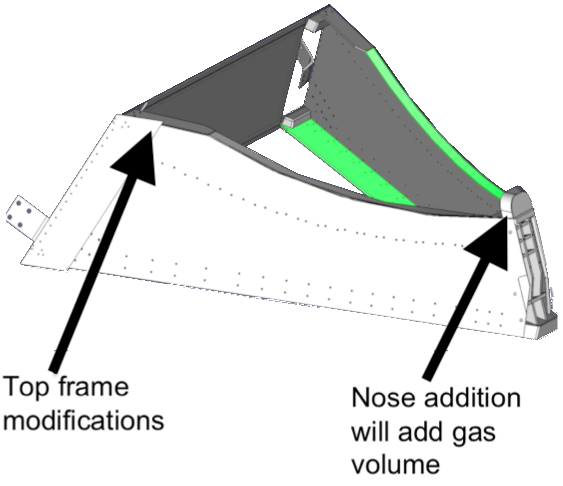
\includegraphics[width=1.0\columnwidth,keepaspectratio]{img/boxCut.png}
	\caption{The LTCC frame modifications. The side-walls had to be cut near the top part of the box from their original
            spherical to a flat outline. The last 3 mirror set had to be relocated. At the bottom of the box, a stainless steel
            nose window support was added to increase the gas volume}
	\label{fig:boxCut}
\end{figure}


\paragraph{Nose Addition}

In the original design the upstream window followed the spherical curvature of the frame sidewalls. In the new design, the window is left to inflate
to enlarge the gas volume in order to increase the number of Cherenkov photons. In addition, a ``nose'' support (see Fig.~\ref{fig:boxCut})
has been designed and built to increase the gas volume.
The nose dimensions have been optimized to provide the best support while at the same time maximize the gas volume increase. The gas increase
of the final configuration is shown in Fig.~\ref{fig:noseVolume}.

\begin{figure}[hbt]
	\centering
	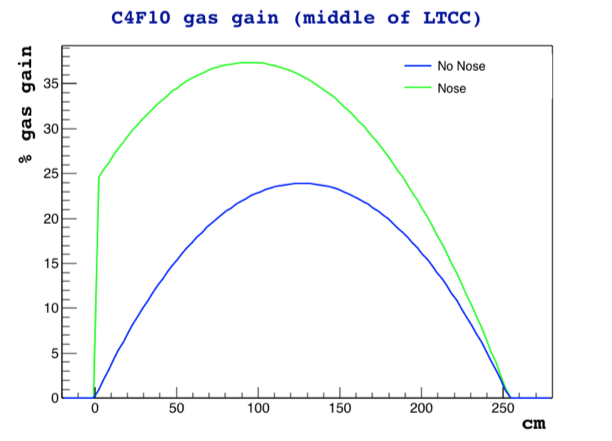
\includegraphics[width=1.0\columnwidth,keepaspectratio]{img/noseVolume.png}
	\caption{The gas volume percentage gains with and without the nose addition compared to the CLAS6 configuration. Blue: the increase due
	          to the window inflation. Green: the additional increase due to the nose addition. }
	\label{fig:noseVolume}
\end{figure}


\paragraph{Back-wall and Connectors}
In the original implementation both the high voltage and signals connectors that link the PMTs inside the hermetical box and the electronics were not
hermetical. Epoxy has been used to minimize the leaks from these connectors.
During the refurbishment the patch panel had been re-design to accommodate hermetical connectors. This involved rebuilding the back wall entirely.

The new back wall design is shown in Fig.~\ref{fig:backWall}. The wall is supported by stainless steel bars that enclose a panel made of foam enclosed by
thin aluminum sheets to minimize the radiation length.
The new patch panels provides 3 connectors for each PMTs: one for High Voltage and two for an identical signal coming from the modified PMT base.
The new connectors are hermetical to eliminate gas leaks in the patch panel.

\begin{figure}[hbt]
	\centering
	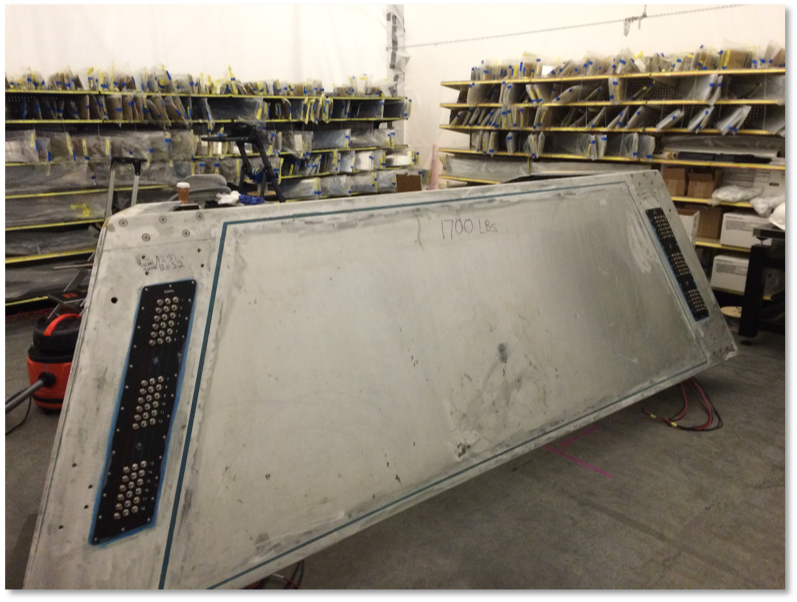
\includegraphics[width=1.0\columnwidth,keepaspectratio]{img/backWall.png}
	\caption{Top view of the back-wall of the LTCC. A stainless steel bar encapsulate a sandwich wall of aluminum and foam. On the left and right side
            of the frame a new patch panel allow for 3 hermetical connectors (1 HV, 2 signals) from each PTM. }
	\label{fig:backWall}
\end{figure}


\paragraph{Mirror Support Spine}

\begin{figure}[hbt]
	\centering
	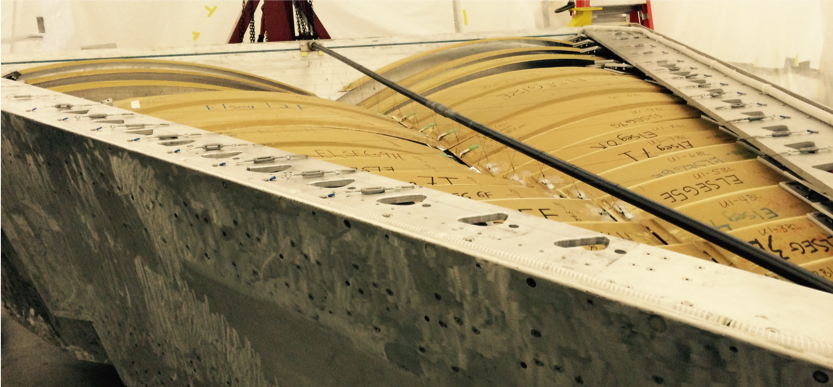
\includegraphics[width=1.0\columnwidth,keepaspectratio]{img/spine.png}
	\caption{Top view of the back-wall of the LTCC. A stainless steel bar encapsulate a sandwich wall of aluminum and foam. On the left and right side
            of the frame a new patch panel allow for 3 hermetical connectors (1 HV, 2 signals) from each PTM. }
	\label{fig:spine}
\end{figure}


- Seal the box from the inside
- Window: glue + sealant




